\documentclass[xcolor=pdftex,dvipsnames,table,handout]{beamer}
\usetheme{Madrid}
\usepackage{color}
\usepackage{url}

\title{Title of the paper/book chapter}
\subtitle{Authors, year, publisher}
\author[]{your name}

\institute[Unit ?]{Department of Computer Science\\ 
National Tsing Hua University}

\date{\today}

\begin{document}
\begin{frame}
  \titlepage
\end{frame}

\begin{frame}  \frametitle{Title of the slide}
\begin{block}{Block of information}
\begin{enumerate}
\item item 1
\item item 2
	\begin{enumerate}
	\item list 1
	\item list 2
	\end{enumerate}
\end{enumerate}
\end{block}

\begin{itemize}[<+->]
\item For more details, please see 

\url{https://www.overleaf.com/learn/latex/Beamer_Presentations:_A_Tutorial_for_Beginners_(Part_1)\%E2\%80\%94Getting_Started}
\item item 2
\item item 3
\end{itemize}
\end{frame}

\begin{frame}  \frametitle{Use columns}
\begin{columns}
\column{2.5in}
\begin{definition}[1.1]
A point $x^{*}$ is a {\color{red} global minimum} of $f(x)$ if for all $y$ in the feasible set of $x$, $$f(x^{*}) \leq f(y).$$
\end{definition}
\begin{definition}[1.2]
A point $x^{*}$ is a {\color{red} local minimum} of $f(x)$ in the neighborhood $N(x^{*},r)$ if for all $y \in N(x^{*},r)$, $$f(x^{*}) \leq f(y).$$
\end{definition}
\column{2in}
\centering
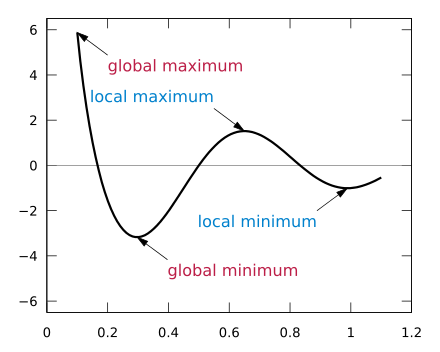
\includegraphics[width=2in]{minimum.png}
\end{columns}
\end{frame}

\end{document} 